\graphicspath{ {./images/} }
\begin{problem}%
{Космический мусорщик}%
{\textsl{стандартный ввод}}%
{\textsl{стандартный вывод}}%
{2 секунды}%
{64 мегабайтa}{}

В околоземном космическом пространстве накопилось много мусора, поэтому ученые сконструировали специальный аппарат - ловушку для космического мусора. Для того, чтобы хорошо собирать мусор, этот аппарат должен двигаться по достаточно сложной траектории, сжигая собранный по пути мусор. Ловушка может передвигаться в пространстве по 6 направлениям: на север (N), на юг (S), на запад (W), на восток (E), вверх (U) и вниз (D). Движением ловушки управляет процессор. Программа движения задается шестью правилами движения, которые соответствуют каждому из указанных направлений. Каждое такое правило представляет собой строку символов из множества {N, S, W, E, U, D}. \\ 

Команда ловушки есть пара из символа направления и параметра - целого положительного числа $M$. При исполнении такой команды ловушка в соответствии со своей программой выполняет следующее. Если параметр больше $1$, то она перемещается на один метр в направлении, которое указано в команде, а затем последовательно выполняет команды, заданные правилом для данного направления, с параметром меньше на $1$. Если же параметр равен $1$, то просто перемещается на один метр в указанном направлении. \\

Пусть, например, заданы следующие правила:

\begin{center}
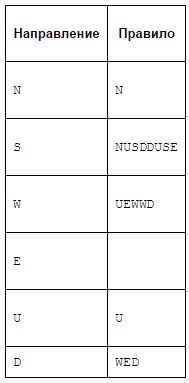
\includegraphics{space.jpg}
\end{center}

Тогда при выполнении команды S(3) мусорщик выполнит следующие действия: \\ 

1) переместится на 1 метр в направлении S \\
2) выполнит последовательно команды N(2), U(2), S(2), D(2), D(2), U(2), S(2), E(2). \\

Если далее проанализировать действия мусорщика при выполнении команд из пункта $2$, получим, что в целом он совершит следующие перемещения: \\

$SNNUUSNUSDDUSEDWEDDWEDUUSNUSDDUSEE$ \\

По заданной команде определите, какое общее количество перемещений на один метр совершит ловушка при выполнении заданной команды. В приведенном примере это количество равно $34$.

\InputFile

Первые шесть строк входных данных задают правила для команд с направлением N, S, W, E, U и D соответственно. Каждая строка содержит не более $100$ символов (и может быть пустой). Следующая строка содержит команду ловушки: сначала символ из множества {N, S, W, E, U, D}, затем пробел и параметр команды - целое положительное число, не превышающее $100$.

\OutputFile

Выведите единственное число - количество перемещений, которое совершит ловушка. Гарантируется, что ответ не превышает $10^9$.

\Examples

\begin{example}
\exmp{
N
NUSDDUSE
UEWWD

U
WED
S 3
}{%
34
}%
\end{example}
\end{problem}
